%%This is a very basic article template.
%%There is just one section and two subsections.
\documentclass[pdftex,11pt,a4paper]{article}

\usepackage{fancyvrb}
\usepackage[margin=1in]{geometry}
\usepackage{graphicx}
\usepackage{float}
\usepackage{indentfirst}
\usepackage{url}
\usepackage{amssymb, amsmath}
\usepackage[T1]{fontenc} % font encoding
\usepackage[utf8]{inputenc} % input encoding
\usepackage[english]{babel} % keyword translation and hyphenation
\usepackage{lmodern} % lmodern looks better than cm-super
\usepackage{moreverb}
\usepackage{soul}
\usepackage[table]{xcolor}% http://ctan.org/pkg/xcolor
\usepackage[none]{hyphenat}%%%%
\usepackage{color, colortbl}
\usepackage[first=0,last=9]{lcg}

\definecolor{Gray}{gray}{0.9}
\definecolor{LightCyan}{rgb}{0.88,1,1}

\newcommand{\ra}{\rand0.\arabic{rand}}

\begin{document}

\title{Model transformation tools -- a comparision between 3 different tools}
\date{April 23}
\author{Petter Barvik}

\maketitle

\abstract{}
\noindent Model transformations play a key role in Model Driven Development.
There are quite a few model transformation tools open to the public that
delivers a model transformation environment. This can be tools that are
integrated with the Eclipse Modelling Framework or stand alone tools that do not
use any framework. This paper focus on three tools that delivers an environment to
create and execute model transformations. AGG and Henshin provides a model
transformation environment, based on graph transformations they provide a left
and a right hand side to create and modify rules. ATL provides a textual editor
that is integrated with OCL to specify model transformations. For each tool we
will go through the process from changing a model written in one modelling
language to another modelling language. We want to see how this process is
handled amongst the three tools and do a comparison amongst the tools.

\newpage
\section{Introduction}

\noindent Model Driven Engineering (MDE)\cite{France2007} thrives to raise the
level of abstraction in program specification and increase automation in program
development. The main idea in MDE is to use models at different levels of
abstraction when developing software applications. This leads to a higher level
of abstraction in application code and problem specification. This level of
abstraction is obtained either through extensive use of models to describe some
design patterns in a software application or through use of standardized
models. The first option is probably an element of MDE that is more common
among software engineers, where a developer use models as a reference point to 
implement some aspect. Unified Modelling Language\cite{UML} is an example of a
modelling language often used to describe system design patterns in an application
domain. The second principle of Model Driven Engineering is to increase
automation in program development, and to obtain this we use model
transformations. \\
\indent A model transformation is when we change an instance of the source
language to an instance that conforms to the target language. We can
distinguish these operations into either endogenous or exogenous model
transformations. In an endogenous model transformation we take one model
expressed in a language and produce a model expressed in the same language.
While in an exogenous model transformation we start with a model
expressed in one language and translate this into a model expressed in another
modelling language. It is essential that these models are consistent. This is
obtained through the use of metamodels. A metamodel is a description of a
modelling language, where it defines elements that are used in the model.
A model transformation can produce two different kind of output models. The
first one is code generation, often referred to Model to Text(M2T)
transformation, and it takes one model and produces implementation code. This
is convenient if for example a software engineer wants to produce source code
from a given model. 
The latter is often referred to Model to Model(M2M) transformations. M2M
transformations take a model as input and produces a model as output. In this
article we try and go into depth for some model to model transformation tools.
These tools are The Henshin project\cite{Henshin}, Attributed Graph Grammer
System (AGG) \cite{AGG} and ATLAS Transformation Language (ATL) \cite{ATL}.
Henshin and AGG is build around the algebraic concepts of graph
transformations. Whereas ATL transformation language is a textual based
transformation language that relies on manual coding to create model to model
transformations. In this paper we will look at a specific example of a model to
model transformation, where we want to change an Activity diagram
to a Petri Net model and evaluate how this example performs for different
tools. When we have applied this example to the different tools, we will
evaluate the approaches to model transformation for these tools. In the next
section, we will shortly describe the two models that are involved in this
model to model transformation. Then in chapter 2 we will look at what graph
transformation is. Model transformations is still a subject of research, and to
use graph transformation or graph rewriting is the most common technique used at
this moment to handle model to model transformation problems for graph based
models. In chapter 3, 4 and 5 we will look at these three different tools.
We will briefly consider how to edit and create model transformations for the
different tools. If its either a graphical editor or a textual based editor. We
will also describe how these three tools handle consistency and metamodels. And
how to specify transformation rules for each tools. We will also describe how
the different tools administrates the different transformation rules and how
the rules are applied to an instance model. And in the final chapter, we will
evaluate these tools. Where we will look at strength and weaknesses. But before
we go into depth in these tools, we will present the example scenario for this
paper.

\subsection{Problem specification}
\noindent The task was to take a certain instance of a model to model
transformation, in this case translating an activity diagram, written in the
language UML, and transform it to a Petri Net model. We initialize the
metamodels to make sure that the models remain consistent. These metamodels are
represented in the Ecore model\cite{Steinberg2009}. The Ecore model is used to
represent models in Eclipse Modelling Framework (EMF) \cite{Steinberg2009}.
Models and metamodels created in EMF needs to conform to the Ecore Metamodel.
You could say that this makes Ecore a meta-metamodel, since the two metamodels
below are represented in Ecore. The reason why we represent the target and the
source metamodels in Ecore in this sections is because two of the tools support
metamodels written in Ecore.

\begin{figure}[H]
	\centering
	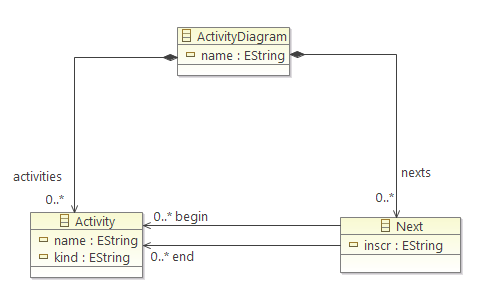
\includegraphics[scale=0.8]{figures/ActivityMetamodel.png}
	\caption{Metamodel of Activity Diagram.}
	\label{fig:ActivityMetamodel}
\end{figure}

The metamodel of an activity diagram has an arbitrary number of activities and
next elements. Figure~\ref{fig:ActivityMetamodel} describes that an activity
element can have a name and a kind. Example of activity types can be decision or
simple. The next element can have an inscription and has the property to either
start or end activities. The collection of activities and next elements have to
have an activity diagram that they belong to. Now we have defined the metamodel
that the source model should conform to. To keep consistency between the models
we need to have a metamodel for the target model.

\begin{figure}[H]
	\centering
	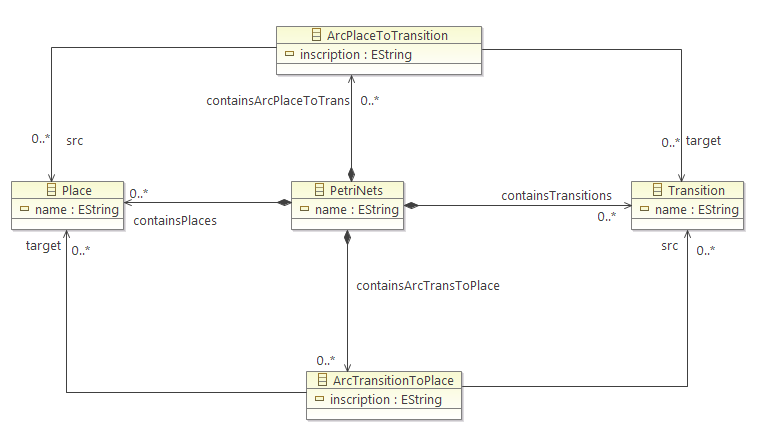
\includegraphics[scale=0.7]{figures/PetriNetsMetamodel.png}
	\caption{Metamodel of Petri net.}
	\label{fig:PetriNetsMetamodel}
\end{figure}

The metamodel for Petri net consist of places and transitions. A Petri net
instance must have a place connected to a transition or the other way around.
But a Petri net can never have two of the same types connected with each other.
To solve this, the Petri net metamodel has two nodes that specify if the
connection is between a place and a transition or a transition and a place.

These two metamodels can be used as both source and target metamodel for both
Henshin and ATL, while AGG does this a bit more differently. In AGG we have to
initialize a type graph that contains both source and target metamodel instead
of having these metamodels in separate files. We will look at this type graph
in more depth in chapter 3.

\section{Graph based approach to Model Transformation}
\noindent One common approach to model transformations is by graph
transformations, also referred to as graph rewriting. Graph rewriting can be
implemented with an algebraic approach, which is based on category
theory\cite{Barr1990}.

\begin{figure}[H]
	\centering
	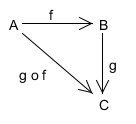
\includegraphics[scale=0.7]{figures/categoryTheory.png}
	\caption{Collection of objects A,B and C.}
	\label{fig:categoryTheory}
\end{figure}


In category theory there are a collection of objects and arrows. These arrows
are also called morphisms. In figure~\ref{fig:categoryTheory} we have a
collection of objects A, B and C and morphisms f, g and g $\circ$ f. And for the
purpose of this paper, the collection of objects are graphs and the arrows are
graph morphisms. This is also very typical when writing papers to explain the
concepts of graph transformations, where these objects are represented as
graphs, and arrows are represented as morphisms between graphs. Category theory
can then be used to formalize the concepts at a high level of abstraction.

\subsection{The Algebraic Approach}
\noindent This approach are based on the concepts of composing graphs, modelled
by pushouts of graphs and graph morphisms. This pushout approach comes in
different variants, and we will look at two of these, namely the
double-pushout (DPO) approach and the single pushout (SPO)
approach\cite{Loewe1997,Ehrig1997}.

\indent Historically, the first of the algebraic approaches to graph
transformations, the double-pushout, was first introduced at the Technical
University of Berlin in the early seventies by H. Ehrig, M. Pfender and H.J.
Schneider\cite{INSPEC:606170}. They tried to generalize Chromsky grammars from
strings to graphs. This allowed to define a graph rewriting step by the use of
two gluing constructions. And by applying a graph rewriting step for the
double-pushout approach is a pair of morphisms in the category of graphs where
the arrows represents total graph morphisms, \linebreak\mbox{L $\longleftarrow$
\ K $\longrightarrow$ R}. This is true for each application rule in a graph
transformation for the double-pushout approach. Where the graph K represents the
common part and the two morphisms \mbox{L $\longleftarrow$ \ K} and \mbox{K
$\longrightarrow$ R} use the algebraic construction, pushout to apply an
application rule for a rewriting step. Hence the name double pushout and the use
of two rewriting conditions.

\subsection{Transformation Rules}
\noindent For a transformation language to be able to execute graph
transformations a set of application rules needs to be defined. Through these
rules, a transformation interpreter can act accordingly. These rules are often
referred to as Productions. For graph transformations, there can be an arbitrary
number of rules. Its truly up to the users how they want to translate a
language and how many rules that is needed to acquire this. Each rule consists
of a left hand side (LHS) and a right hand side (RHS), also often referred to as
pattern graph and replacement graph. The pattern graph represents a subgraph of
the model that is going to be translated, namely the host graph. For these
productions to execute, there has to be some control mechanism, namely the
transformation unit.


\subsection{Transformation Units}
\noindent In graph transformation, there has to be a control mechanism that
administrates these productions. These control mechanisms are also called
transformation units. These units controls the order that the transformation
rules are executed. The most basic transformation unit is a rule itself which
corresponds to a single application of that rule. But in most cases, a
transformation unit will have to control several rule applications. 

\subsection{Execution of rules}
\noindent The basic idea for graph transformation for both the double-pushout
approach and the single pushout approach is to apply an application rule
\mbox{r: L $\longrightarrow$ R}. Where the rule represents a single rewriting
step for graph transformations and L represents the left hand side of the rule and R
represents the right hand side of the rule.

\begin{figure}[H]
	\centering
	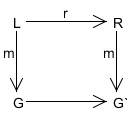
\includegraphics[scale=0.7]{figures/GraphTransformationGeneral.png}
	\caption{The basic idea for graph transformation by applying a rule r.}
	\label{fig:GraphTransformationGeneral}
\end{figure}

For a production rule r, \mbox{G$\xrightarrow{r,m}$G'} indicates a direct
derivation to a derived graph G'. In
figure~\ref{fig:GraphTransformationGeneral}, the graph G' is created by
applying a single pushout for a transformatin rule r. If there is a match m of
nodes and arrows for a subgraph L in a host graph G, then this indicates a
graph homomorphism, mapping elements from the subgraph to the host graph in
such a way that the graphical structure in G is preserved. For each rule r,
there are some algebraic approaches to how we can achieve G'. At this moment
there are four approaches, the double-pushout approach (DPO) \cite{Loewe1997}, the
single-pushout approach (SPO) \cite{Ehrig1997}, the sesqui-pushout\cite{Corradini2006} and
the pullback approach\cite{Bauderon}. Where the two most common approaches used in
graph transformation tools are the DPO and the SPO approach. There is one major
aspect that separate these two approaches, and that is that the DPO approach
has an application condition.

\begin{figure}[H]
	\centering
	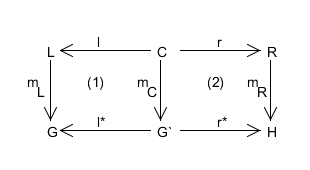
\includegraphics[scale=0.7]{figures/DPO.png}
	\caption{Principles behind the double pushout approach.}
	\label{fig:DPO}
\end{figure}

\noindent This application condition, named the gluing condition\cite{Loewe1997}
consists of two parts. Namely the dangling condition and identification
condition. From figure~\ref{fig:DPO}, the dangling condition requires that if
the transformation rule p specifies the deletion of a node in G, then it must also
specify the deletion of all incoming and outgoing edges of this node in G. By
applying this condition, we can be sure that there are no dangling edges after
deleting a node in G. The identification condition requires that every element
of G that should be deleted by applying a transformation rule p is only present
once in L for each transformation rule p. 

A single transformation rule p in the DPO approach is given by a pair of graph
homomorphisms from a common graph C. This common graph C is formed by taking
elements that are present in both L (LHS) and R (LHS) of a transformation rule
p. The graph G' are created from the graph G, by deleting all elements that is
matched from the pattern graph L, but none in C. To avoid dangling edges,
the gluing condition must be satisfied before deleting these elements. This is
the first part (1) of the DPO approach, namely the deletion of elements. The
second part (2) is insertion of elements. From here we create a graph H off all
nodes and arrows from the replacement graph R that is not presented in the
common graph C. The DPO approach has the possibility to preserve elements from
translating from the pattern graph L and the replacement graph R with the help
of a common graph C.

For the SPO approach on the other hand, deletion has priority over preservation.
Figure~\ref{fig:GraphTransformationGeneral} is a representation of the practices
of the SPO approach. Where nodes that are present in the pattern graph L but not
the replacement graph R are deleted. And the incoming and outgoing edges of the
deleted nodes that are not present in the replacement graph R is deleted.

Now that we have explained some aspects of Graph transformations, we can
describe the three different tools, where both AGG and Henshin is build around
the concepts of graph transformations explained in this section. But first we
will try to explain how ATL utilize the concepts of model transformations. 

\section{ATL Transformation Language}

\noindent ATL\cite{ATL} (ATL Transformation Language) is a model transformation
language and is an answer to the QVT\cite{QVT} standard. It
provides ways to produce a set of target models from a set of source models.
ATL is developed on top of the Eclipse platform and is one of three
transformation engines provided by the Model to Model Transformation (MMT)
project\cite{MMT}. The MMT project hosts Model to Model Transformation
languages. These transformations are executed by transformation engines that are
written into the Eclipse Modeling infrastructure. MMT is a sub project of the
top level Eclipse Modeling Project\cite{EMP}. ATL is maintained by
OBEO\cite{OBEO} and AtlanMod\cite{ATLANMod} and was first initiated by the
AtlanMod team, previously called the ATLAS Group, located at the University of
Nantes in France. The initial version of ATL was created In 2004, where ATL
became part of the Eclipse Generative Modeling Technologies (GMT) \cite{GMT}.
The goal of GMT is to produce a set of research tools in the area of Model
Driven Software Development. The ATL Integrated Development Environment (IDE)
was later promoted for the Eclipse M2M project in January 2007.

There are developed several tools that has support for a declarative
approach to model transformation. For the purpose of this paper, we will explain
this approach with the focus around the Atlas Transformation Language (ATL).
ATL is a hybrid model transformation approach, that is a transformation
language that combines other model to model transformation approaches. For
example, ATL provides transformation rules that can be either fully declarative
or fully imperative or a mixture of both. 

\begin{figure}[H]
	\centering
	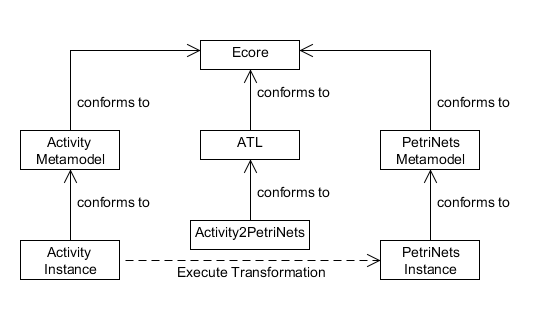
\includegraphics[scale=0.55]{figures/ATL.png}
	\caption{Model transformation process for Activity2PetriNets.}
	\label{fig:ATL}
\end{figure}

Figure~\ref{fig:ATL} gives us an idea of how the ATL transformation from an activity
diagram to Petri net are handled. We want to generate a instance of PetriNets,
that conforms to its own metamodel. This is generated from a source
model, Activity Instance, that conforms to its respective metamodel.
The created transformation Activity2PetriNets is expressed in the ATL
transformation  language, that conforms to its own metamodel. These three
metamodels conform to the metamodel Ecore. So this makes Ecore a metametamodel
to represent the metamodels of Activity, ATL and PetriNets.

ATL has to be configured properly before the user can execute a model
transformation. In this configuration both the location of the source and target
metamodel has to be specified. The user also has to specify what instance model
that should be translated. And lastly the user has to create a new file that can
be specified as the target instance model for the ATL run configuration. The
user can then initiate the transformation by running this as an ATL
transformation.


\subsection{Textual editor}

\noindent ATL can be compared to a programming language, because it is
basically a transformation language that provides a concrete textual syntax. ATL
is a text based transformation language, and is build around the Object
Constraint Language (OCL) \cite{OCL} with some additional predefined functions.
ATL transformations is stored in a file extension called ``.atl'' These ATL
files can contain different kind of ATL units and are defined in its own
distinct ATL file. These different ATL units are ATL modules, ATL queries and
ATL libraries. Libraries can be used to create independent ATL libraries that
can be imported to different types of ATL units. The module unit specifies the
different application rules for a  model transformation. And the Queries are
used when the users want to compute primitive values from the source models.

Now that we have specified these three ATL units, we can describe shortly how
we can use the ATL transformation language to create model to model
transformations. For our case study, we only need the ATL modules. An ATL module
corresponds to a model to model transformation. This unit enables developers to
specify the way to produce a set of target models from a set of source models.
The source and target models of an ATL module must be consistent with their
respective metamodels. 

\subsection{Defining Metamodels}

Defining metamodels for the ATL language is defined by the modelling language
Ecore. Since defining the metamodels are defined the same way as Henshin, see
chapter 4.2.

At first, the user start out with a blank ATL file. Since we are working in
the ATL Integrated Development Environment for Eclipse, we want to start the
document with defining the path to the source and the target metamodel. The
reason for doing this is to achieve auto completion from elements defined in the
Ecore metamodels. This is convenient for the users when creating transformation
rules.  

\begin{figure}[H]
	\centering
	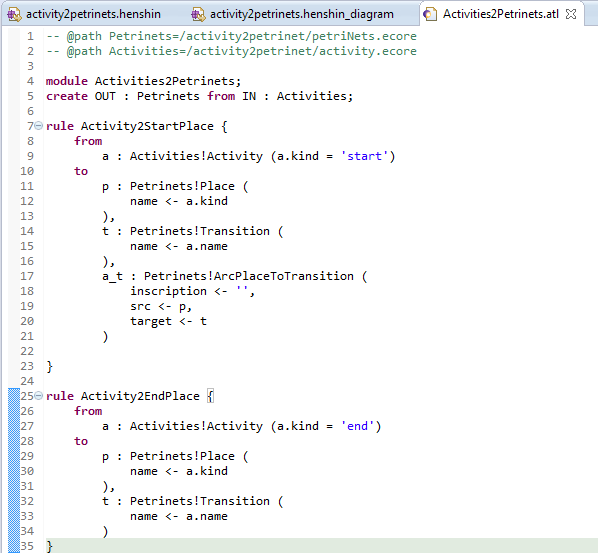
\includegraphics[scale=0.5]{figures/ATLScreen.png}
	\caption{Two simple rules for Activity2PetriNets in ATL.}
	\label{fig:ATL_Screen}
\end{figure}

Next the file is composed of four different elements. The first element is the
header section, where the user can give the module a name and name the variables
corresponding from the source and target models. The module name has to be
identical to the name of the ATL file.

We also need to specify the source and the target metamodel. From
figure~\ref{fig:ATL_Screen} we can see that the target metamodel is initialised 
with the keyword create, and the source metamodel is initialised using the
keyword from. The user can also import some existing libraries if needed. This
import section is however optional. Importing metamodels are handled a bit
differently in ATL compared to Henshin. In ATL the metamodels are imported
explicitly while in Henhsin they are imported implicitly before they can be used
in modifying the transformation rules. For ATL the user has to configure where
both the source and the target metamodel are located through a configuration
page. 

The next element is a set of rules that defines how the target models are
generated from the source models. These rules are used to implicitly match
source elements and produce target elements. In figure~\ref{fig:ATL_Screen} we
have examples of two rules, namely the rule for transforming the start activity
and the rule for transforming the end activity. We can see that for each rule we
specify what we want to translate from and what we want to translate to. We will
describe transformation rules in more details in the next section.

The last element in a ATL module is a set of helper functions. This collection
of helpers can be compared to Java methods. These helper methods can be used to
make the transformation rules easier to read for example.

\subsection{Transformation Rules}

A rule in ATL describes how a target model should be generated from a source
model. In ATL there are three kinds of rules, the type matched rules and the
lazy rules are both fully declarative while the called rules are imperative.
These rules has an input pattern and an output pattern. The input pattern can
have a list of source model elements that is part of a rule in ATL by defining
several input pattern elements. Each input pattern element has to have a
mandatory type that corresponds to a metaclass defined in some metamodel. Each
rule corresponding input pattern can also specify optional conditions that are
expressed as OCL expressions. Both the type and an optional condition specifies
which elements from the source model that is matched for each rule. The output
pattern defines how the target model elements are created from the input model. 

\textbf{The matched rules} provides an declarative approach to
creating transformation rules in ATL. The users can specify from which kinds of
source elements the target elements can be generated from and how the generated
target elements should be initialized. A matched rule finds a match according to
the type of source model element and generate target model elements from these
matches. A new matched rule is defined by the keyword ``rule'' and has two
mandatory and two optional sections. The mandatory sections specifies the input
pattern and the output pattern while in the first optional section the users can
declare and initialize local variables. Note that these variables can only be
used in the scope of each rule. The second optional section includes an
imperative section The type that is introduced in the input pattern conforms to
a meta-element in a metamodel of the source model. This rule will then generate
target elements according to each match in the source model.

Figure~\ref{fig:ATL_Example} shows a simple rule, Activity2StartPlace that wants
to translate Activity source elements to some target elements. This rule
specifies the keyword \textit{from} for the input pattern and \textit{to} for
the output pattern. For this example we want to find matches for one source
element that is of type Activity that conforms to the metamodel Activities. We
also provide additional properties for this input source element, where we only
want to find matches that conforms to the type Activity and has the name
``start''. The rule specifies that we want to generate three target
pattern elements p, t and a\textunderscore t from this matching type. These
generated target elements conforms to the metamodel Petrinets and specifies
that these generated types should generate attributes from the source
pattern element. The generated target model elements is initialized with
attributes from the matched source pattern element. 

\begin{figure}[H]
	\centering
	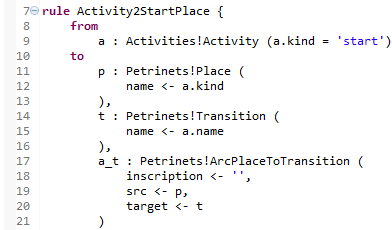
\includegraphics[scale=0.7]{figures/ATL_Example.png}
	\caption{An example of a matched rule in ATL.}
	\label{fig:ATL_Example}
\end{figure}

If applicable the users can add an optional condition for each rule to check for
certain matches for this input element. This condition is expressed as an OCL
expression and gives the user the possibility to restrict the searches of the
source elements. 

The second type of an ATL rule is \textbf{Lazy rules}. These lazy rules will
never be applied when a model transformation in the Atlas Transformation
Language is executed. These lazy rules can only be applied to a model
transformation when they are called from another of the two rules. These lazy
rules are created similar to the matched rules.

The third and final type for an ATL rule is called \textbf{Called rules}. A
called rule has to be called from an imperative section from either a match rule or
from another called rule. A called rule is created similar to a matched rule,
namely with a \textit{rule} keyword. One thing that is special with a called
rule is that it does not have to match source elements from the source model.

\subsection{Execution of an ATL transformation}

Figure~\ref{fig:ATL_Execution} describes the architecture of the transformation
language. From the figure we can see that we have an association between EMF and
Ecore models. This are the metamodels that are expressed using EMF's Ecore
model. These metamodels are then translated through a model handler that
compiles these ecore models to the ATL Virtual Machine. Where these metamodels
can be used both in creating ATL programs and in ATL's internal interpreter. The
ATL compiler translates the ATL file into a new ASM assembler file, that ATL can
use to launch a model transformation. This assembler file contains the
compiled code of the corresponding ATL file.

\begin{figure}[H]
	\centering
	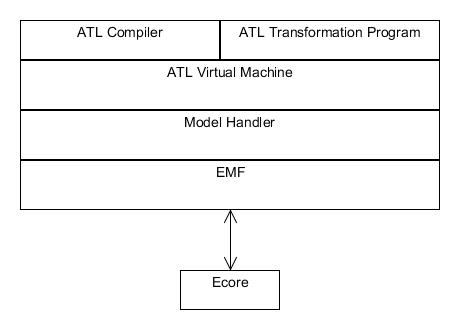
\includegraphics[scale=0.6]{figures/ATL_Execution.png}
	\caption{Internal infrastructure of for ATL.}
	\label{fig:ATL_Execution}
\end{figure}

The default semantics for executing a set of transformation rules specified in
ATL can be described in three phases. See ATL User Manual\cite{ATL_USERMAN} for
more information.

The first phase is an initialization phase. This phase consist of amongst other
things to initialize the trace model and the module of the ATL transformation.
The trace model in ATL has one important function, and that is to create a
trace link that points to the matched source input elements and the
corresponding generated target output elements. The trace model in ATL works as
an implicit tracing mechanism that specifies relationships between the source
element and its corresponding target elements by using a native type called
ASMTransientLink\cite{Wagelaar}. For every time a transformation rule is
matched to a source element, one ASMTransientLink is created. To this transient
link the name of the transformation rule provided together with the source
element and the target elements. These links are added to a collection that is
stored internally for ATL. This means that the users of ATL cannot access these
links after a model transformation has finished executing. However, as shown by
Andr\'{e}s Yie and Dennis Wagelaar\cite{Wagelaar}, that gaining access to these
ATL traces can be done explicitly by creating transformation rules that
generates a tracing model based on the internal tracing information provided by ATL.

The next phase consist of finding matches in the source pattern of the matched
rules. This is done by the ATL transformation engine that searches for valid
matches. A match is valid when all input pattern elements are found amongst
the source model elements and any OCL expression for that matched rule is valid.
The transformation engine also allocates the target model elements based on the
declared output pattern into memory. At this point the target model elements are
only allocated, they are initialized in the final phase. For each match found,
there is created a trace link that has a source link to the matched source
elements and a target link to the generated target elements. The generated
target elements are not given any attributes or properties in this phase. This
phase create target elements from matches found, and create a trace link between
them.

The final phase of for executing an ATL module is to initialize the target model
elements. At this stage each allocated target model element are given
attributes and features that corresponds to the matched rule. The ATL
transformation engine now use the trace links to determine the matched source
elements and the generated target elements. This operation is called
resolveTemp, that returns the reference from the target model elements that
where generated in the second phase and to the corresponding source model
element. Now that these three phases is finished the ATL transformation engine
can execute the imperative code sections defined for the module. 

\section{The Attributed Graph Grammar System}

\noindent AGG is a general development environment for algebraic graph
transformation systems. AGG is provided with a graphical editor for creating
and modifying graphs. The editor provides a graphical user-interface with
several visual editors for applying the principles of graph transformation. It
also has an interpreter and a set of validation tools. AGG is ongoing research
activity of the graph grammar group at TU Berlin. The work on AGG started in 1997.

\subsection{Graphical Editor}
\noindent The graphical editor of AGG, represented in
figure~\ref{fig:AGGScreen}, has several functions to help the user to define
model transformations. In the top left corner of the graphical user-interface
is a tree based editor for defining rules and grammar. This tree based editor
also contains the type graphs and the host graphs. Where the host graph
represents some input model for a model transformation.

Each application rule has two visual editors, representing the left
(LHS) and the right hand side (RHS), or the pattern and the replacement graph.
In the tree based editor containing rules and grammars it is possible to give
rules application conditions. This is convenient if the user wants to have
constrains for the pattern or the replacement graph.

In the tree based visual editor it is also possible to define host
graphs and type graphs. Type graphs is described more in depths in the next
section, but roughly said, the type graph defines elements that can be used in
the host graph. Type graphs defines the abstract models for the host graph and
is similar to how Ecore defines metamodels  for EMF and the Meta Object
Facility (MOF)\cite{MOF}, that is a language for defining abstract syntax of
modeling languages. The users can now create instances from these type graphs.
These instances represents the host graphs and corresponds to its concurrent
type graph.

For the application rules, the user can extend the attributes with Java
expressions. This means that the users can use Java primitives such as strings,
integers or float numbers to form the pattern graph or the left hand side of
the rule. The user cannot bind attributes that is not initialised in the type graph.

In figure~\ref{fig:AGGScreen} there are some node elements and association
elements to the right side of the figure. These are meta elements that are
initialized in the type graph. These meta elements are used to create the host
graph, the different transformation rules and application conditions. The host
graph is not consistent with the type graph, since these meta elements are
initialized in the type graph. Its worth mentioning that both the
node elements and association elements in the figure has been scaled up for the
purpose of this paper.

\begin{figure}[H]
	\centering
	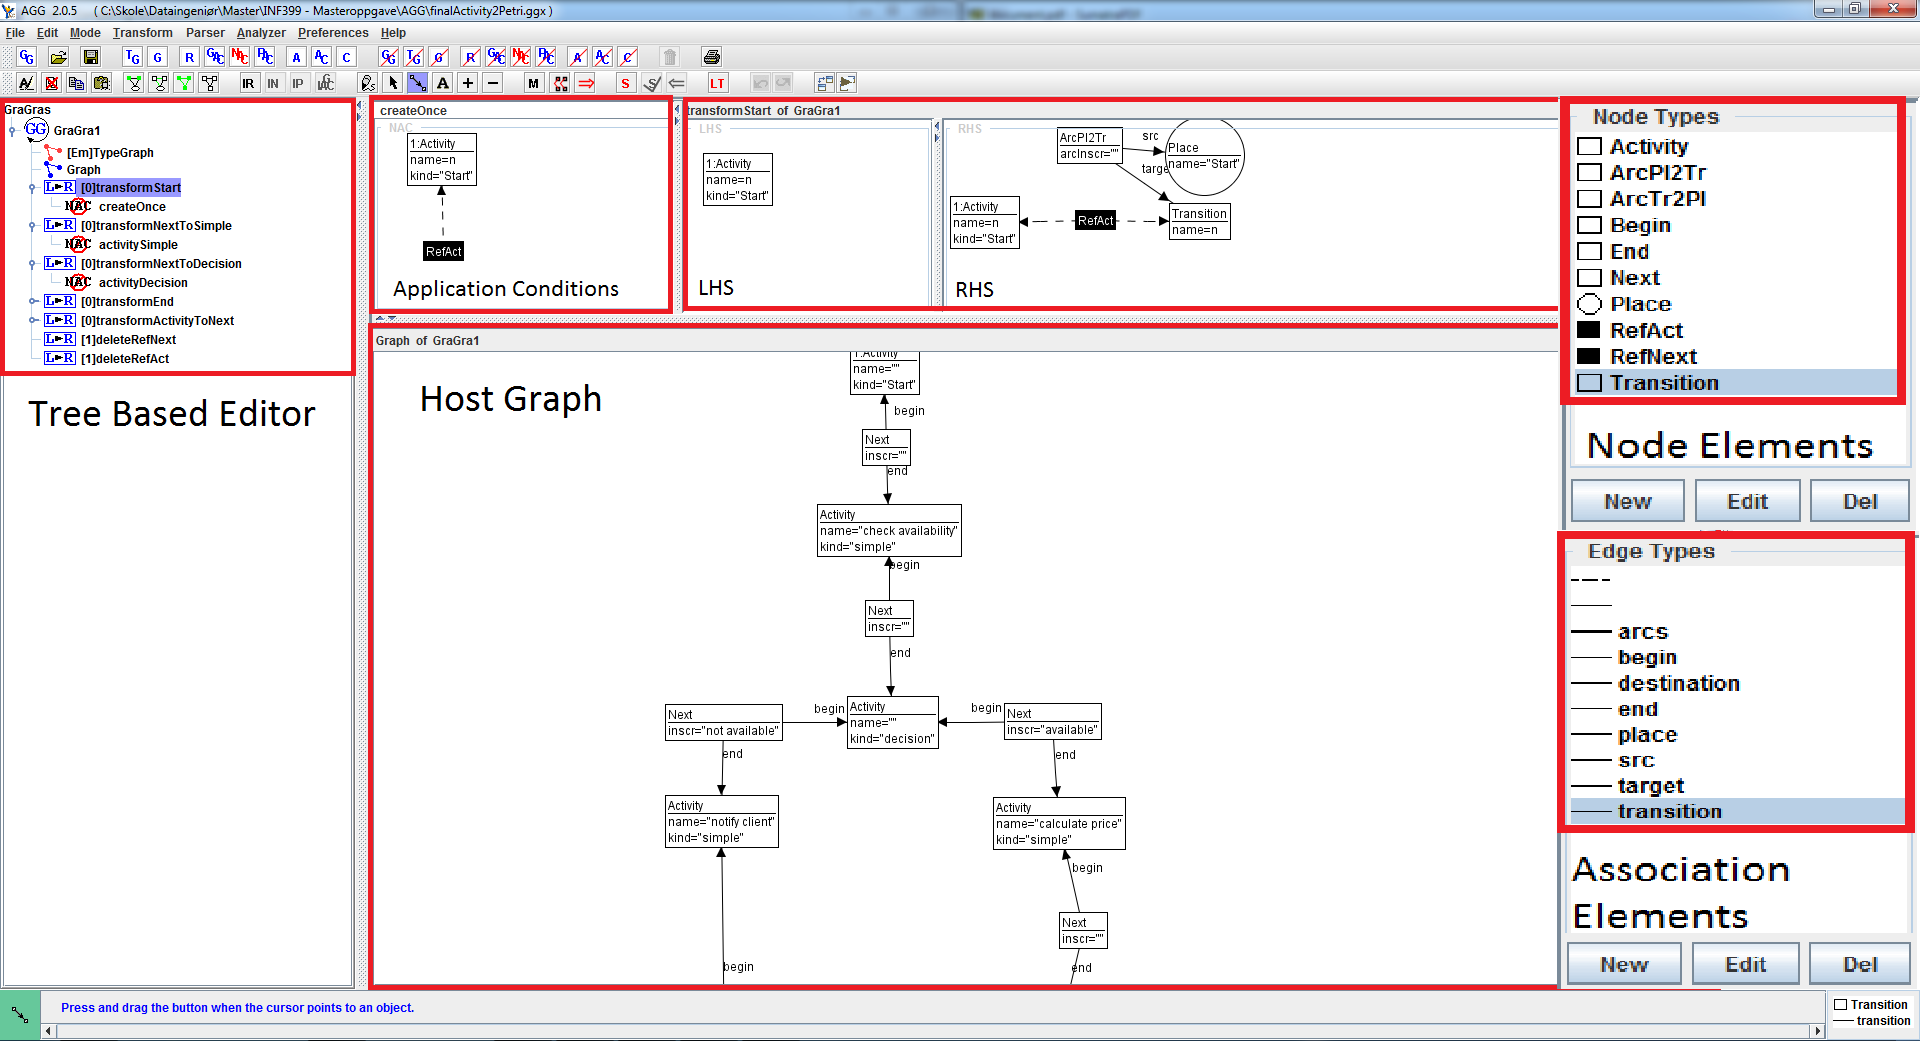
\includegraphics[scale=0.29]{figures/AGGscreen.png}
	\caption{Activity2PetriNets for AGG.}
	\label{fig:AGGScreen}
\end{figure}

\subsection{Defining Metamodels}

\noindent Before the host graphs can be created, we have to initialise the AGG
tool with the metamodels. In AGG both the source and the target metamodel are
defined in a common type graph. This type graph represents the abstract syntax
for the host graph. If we want to prepare an AGG graph for a transformation, we
create a single type graph with references between elements of both source and
target metamodel. This way, when the application rules is executed, we can
choose to keep both the source graph and the references between these elements.
The references and source graph can be deleted through a cycle of transformation rules.

\begin{figure}[H]
	\centering
	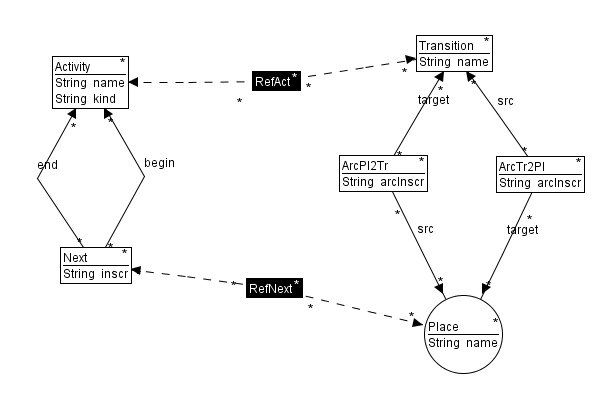
\includegraphics[scale=0.7]{figures/AggTypeGraph.png}
	\caption{Type graph for activity diagram and Petri net in AGG.}
	\label{fig:AggTypeGraph}
\end{figure}

\indent For the type graph, the user must define nodes and arrows for each meta
element for both the source and target model. These nodes and arrows can also
have attributes. Nodes represents elements from the two modelling languages and
arrows represents the associations between these elements. In the type graph we
want to distinguish between associations and references, and therefore we
represent references as a dashed edge. These dashed edges are not given any
attributes, and that is because we want these edges to represent what the
targeted element was translated from. From figure~\ref{fig:AggTypeGraph} we can
see that a RefAct node is defined and is connected between the activity
element and the transition element. The same initialisation is defined between
the next element and the place element. For AGG type graphs there is a
multiplier condition for the edges. This means that there can be an arbitrary,
or a zero to many number of instances of these relations in the host graph.

\subsection{Defining Transformation Rules}
Now the type graph has been initialised and the instance graph of the
source model has been created. But to be able to translate to a target model,
we need to create a set of transformation rules. A transformation rule
require an unique name and a LHS graph and a RHS graph. 

\begin{figure}[H]
	\centering
	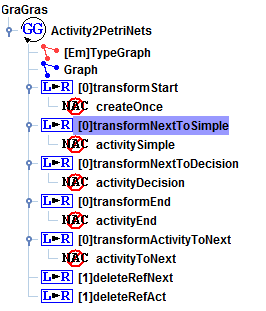
\includegraphics[scale=0.7]{figures/AGGTreeBasedEditor.png}
	\caption{Tree based editor for transformation rules.}
	\label{fig:AGGTreeBasedEditor}
\end{figure}

Whenever changes are made in the two graphs, AGG checks if the LHS or the RHS
conforms to the type graph. The user is unable to insert elements in the two
graphs that are not initialised in the type graph and the users are not allowed
by AGG to create associations between nodes that are not initialised in the type
graph. This is how AGG keep the source and target model consistent. In
figure~\ref{fig:AGGTreeBasedEditor} we can see the tree based editor in AGG,
that provides the type graph, the host graph and a list of application rules.
When a new application rule is created, both the LHS and the RHS of this new
rule is initialised. The users can then insert elements in both the LHS and the
RHS depending on how the source model should be translated. 

\begin{figure}[H]
	\centering
	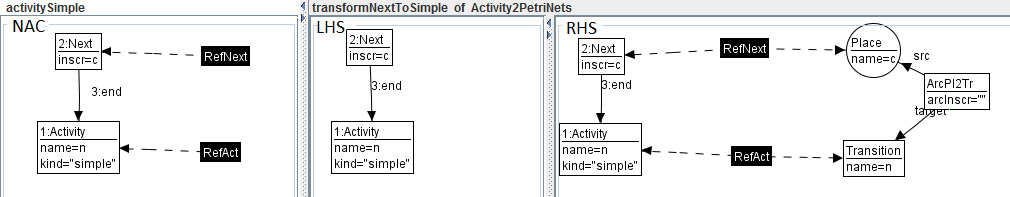
\includegraphics[scale=0.5]{figures/LHSvsRHSAGG.png}
	\caption{Tree based editor for transformation rules.}
	\label{fig:LHSvsRHSAGG}
\end{figure}

Figure~\ref{fig:LHSvsRHSAGG} is a representation of the rule
transformNextToSimple, with both the LHS and the RHS. Each rule can also
contain application conditions. These can either be Positive Application
Conditions (PAC) or Negative Application Conditions (NAC).
Figure~\ref{fig:LHSvsRHSAGG} has a NAC, activitySimple that makes sure that the
LHS of the rule is translated only once for each pattern match found in the
host graph. Through the use of these application conditions, the users can
create restrictions to how each transformation rule should handle pattern match
in the host graph. Each transformation rule can have multiple application
conditions attached.

\subsection{Administrating Transformation Rules}

By default, the control mechanism for administrating the transformation rules
are set to deterministically. This means that the transformation rules are
executed at random. This option is quite useful if the set of transformation
rules are independent of each other. AGG also provides other ways of applying
rules. These are transformation by applying rule layer or by sequences. When the
transformation is set to be applied by rule layers, then the user can add a
number to the different rules. This layer number will range from 0 \ldots n,
where the lowest number is the first layer and therefore the has first
priority. If there are many rules with the same layer number, then these rules
will be internally transformed deterministically. If the rules are applied
by sequence then the rules will be applied from the first element in the tree
based editor and applying the rest of the rules in sequence.

\subsection{Translating the Host Graph}

Now that we have defined the type graph and created the rules it is time to try
and translate the host graph. The preferred option on how the rules should be
applied has also been set. The user can now either press Start Transformation or
do the transformation one step at the time. When the user use the first option
AGG will apply one rule at the time until there is no more matches to be found.
When AGG cannot find any more matches, the host graph is either correctly
translated or there are errors in the rules. 

The user can also execute the transformation step by step. This will give the
user the same result as the first option, but now the user can do one match at
the time for each rule. 


\section{The Henshin Project}

\noindent The Henshin project\cite{Henshin} provides a model transformation
language and an editor for defining model transformations for the Eclipse
Modelling Framework \cite{Steinberg2009}. The Henshin project provides a
transformation language that has support for both endogenous and exogenous
model transformations and a provided graphical syntax. With the help of a
graphical editor, it provides the user with an intuitive way of representing
transformation rules. The Henshin Editor is build on the Eclipse Modelling
Framework and is integrated as an Eclipse plugin. The Henshin Editor was first
developed in a student project at Technical University of Berlin in 2010, and
extended in the bachelor thesis \cite{JohannSchmidt} of Johann Schmidt and the
master thesis \cite{AngelineWarning} of Angeline Warning.

\subsection{Graphical Editor}
\noindent Henshin model transformation language is a plugin for the Eclipse
Integrated Development Environment\cite{Eclipse}. The Henshin project provides
the users with a graphical editor to create and modify model to model
transformations. 

The users start out with using the Eclipse wizard to create an empty Henshin
document. The Henshin document is based on the commonly known Extensible Markup
Language (XML)\cite{XML}. If applicable a Henshin diagram file can be created
based on the Henshin file. This gives the users an intuitive approach to
creating model transformation rules.

The Henshin transformation file is represented in a tree based editor in
Eclipse called Henshin Model Editor. In this tree based editor it is possible
to include metamodels for both the source and the target model, represented in
figure~\ref{fig:Henshin_TreeEditor}. This figure represents the Henshin
Model Editor, where the different transformation rules for this case study is
presented. From this figure we can see that there is a Module element called
activity2Petrinets. This Module element will always be the root element for a
Henshin model transformation. This Module element contains all the user created
rules for performing a model transformation in Henshin. There is also two
external Ecore models included in the editor, more specifically the two
metamodels. These metamodels are created based on the EMF standard for creating
models and are independent of one and another.

\begin{figure}[H]
	\centering
	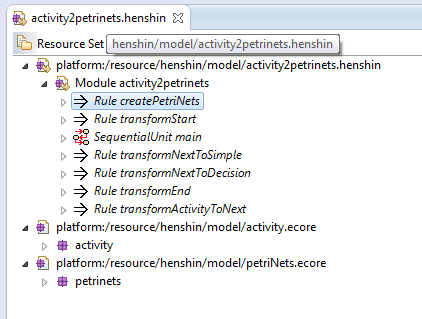
\includegraphics[scale=0.7]{figures/Henshin_TreeEdtiro.png}
	\caption{Tree Based Editor for rules in Henshin.}
	\label{fig:Henshin_TreeEditor}
\end{figure}

\subsection{Defining Metamodels}

The Henshin language requires a source and a target metamodel to be able to
perform model transformations. The target metamodel can either be the same as
the source metamodel or defined in another modelling language. Either way, before
the users can start creating transformation rules, the metamodels has
to be defined. To define these metamodels, Henshin use Ecore, that is
provided with the Eclipse Modeling Framework\cite{Steinberg2009}. Ecore models
can either be created using a tree based editor, called Sample Ecore Model
Editor or by using a graphical editor. While the graphical editor is optional,
the tree based editor is mandatory for creating Ecore models, since this is the
actual Ecore model. 

First the user has to create an EPackage element in the newly created Ecore
model. This EPackage is what Henshin searches for when the user want to import
an Ecore model. This EPackage element can have several child elements, like for
example EClass, EEnum and EData type. For our case study we only needed the
EClass element to create the nodes for the metamodels. And for each EClass
element the users can create EReference elements that can be connected with
other EClass elements. This means that an EReference element defines relations
between the nodes for the metamodels. To give an EClass element properties, the
user can create an EAttribute element. This element can be typed, either by a
predefined list of types or by defining user created EData types. For the
purpose of this case study we only needed to name the different nodes and
therefore we only needed the data type EString. Through the use of these Ecore
elements, we can create the two metamodels from
figure~\ref{fig:ActivityMetamodel} and figure~\ref{fig:PetriNetsMetamodel} from
problem specification in the first chapter.


\subsection{Defining Transformation Rules}

\noindent Now we have defined the source and target metamodel, and imported
both of the metamodels EPackages into the henshin model. We can now use elements
from the two metamodels to create transformation rules in the henshin model
language. In Henshin, objects are referred to as nodes and links between objects
as edges. From the metamodels these nodes represents the EClass elements and
edges is a EReference between these EClass elements. A collection of these nodes
and edges form a graph. This graph is what represent a transformation rule in
Henshin. It is also possible to define variables for each rule. These variables
can then be used to pass along attributes amongst nodes inside the
graph. 

Each transformation rule in Henshin will have two graph assigned.
These two graphs represent the LHS and the RHS of the rule. One thing that is worth mentioning is
that when working with the graphical editor, these graphs are unavailable for
the users to create or modify. Henshin handles assign the LHS and the RHS
through the use of stereotypes. Each rule can be represented as a graph in the
graphical editor. Figure~\ref{fig:HenshinScreen} is a visualization of the
graphical syntax of a specific transformation rule in Henshin.

\begin{figure}[H]
	\centering
	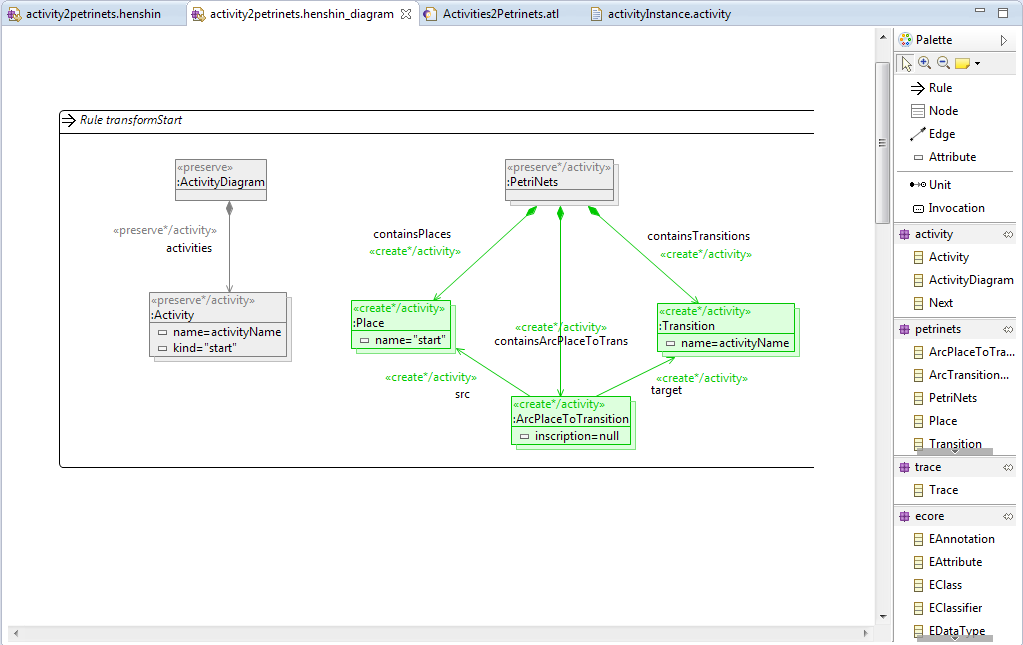
\includegraphics[scale=0.5]{figures/Henshin_Screen.png}
	\caption{Activity2PetriNets for Henshin}
	\label{fig:HenshinScreen}
\end{figure}

This rule is responsible for handling the start element for an activity.
On the right side there is a palette that contains Henshin elements and
different EPackages. The first two EPackages contains elements from the
metamodels we created. The next two EPackages are other models that can
be imported into Henshin. The Henshin Trace model is an EMF model that is used
to keep track of the translated elements during the transformation. This model
consist of a single class Trace, that has two references called source and
target. These references are of type EObject and therefore can refer to any EMF
object. This trace object can be used for all imported models used
in Henshin, since these models has to be defined from the Ecore model. Through
the use of the elements in the palette on right side of the window, the users
can create and modify elements. 
The Rule, Node, Edge and Attribute elements are used to define the different
transformation rules in Henshin. A new transformation rule in Henshin always
have to start with creating a new Rule element. Inside this Rule element the
users are free to create nodes, and connect these nodes with edges. At
all time Henshin makes sure that the created nodes and edges conform to their
corresponding models. The Attribute element can be used if attributes are
defined for the classes that are imported. The Unit element we will come back to
in the next section.

\indent Henshin distinguish elements between the LHS and the RHS through the
use of predefined stereotypes, or action types. Henshin automatically delegates
these elements to the RHS or the LHS from these action types. If the action type
consist of the sequence <<create>>, Henshin knows that this element should be
part of the replacement graph, or the RHS. While on the other side, the sequence
<<delete>> should be part of the pattern graph, or the LHS. The <<preserve>>
sequence is a bit more special, because nodes or edges in Henshin that is of
this action type should be part of both the LHS graph and the RHS graph. This is
done by putting the preserve element in both graphs and then create a mapping
between these two elements to inform the Henshin Interpreter that this is the
same element.

Henshin also has support for application conditions. The action types <<forbid>>
and <<require>> are used for defining Negative Application Conditions (NACs)
and Positive Application Conditions (PACs). These actions are supported for
nodes, edges and attributes. Figure~\ref{fig:HenshinAction} is a representation
of how the users can choose amongst these action types.  

\begin{figure}[H]
	\centering
	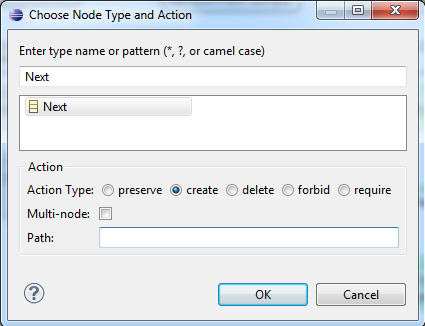
\includegraphics[scale=0.5]{figures/Henshin_Action.png}
	\caption{Action types for a Node.}
	\label{fig:HenshinAction}
\end{figure}

The ``Multi-node`` is a very special Henshin action type. This Henshin
feature gives the users the possibility to create nested multi-rules. This
concept used to be defined as an amalgamation unit in Henshin, but this feature
was changed to give users the opportunity to create rules inside rules. A
multi-rule action type would then be changed to <<create*>>, where the star
informs Henshin that this is a multi-rule. The Path option gives the users
the opportunity to give name this multi-rule. Multi-rule can be very useful if
there is a pattern in the instance graph that is matched more than once. The
users can then use this nested multi-rule concept to match and apply this rule
as often as possible.

\subsection{Transformation Units}
Transformation units in Henshin are used to administrate the different
transformation rules. There are several different units in Henshin that all have
different properties. It is important to mention that a rule is a unit,
since it inherits from a unit in the Henshin metamodel. This means that it is
unnecessary to create a unit in Henshin if our model transformation only
consist of one transformation rule. But if there are defined several
transformation rules there has to be a control mechanism that determines how
these transformation rules should be applied. A Independent Unit is a good
solution if the order of applying the transformation rules is not important.
But if the transformation rules follows a very strict pattern and are dependent
of other rules, then a sequential unit are a safe way to apply rules. The
sequential unit forces Henshin to apply rules in a given order.
Figure~\ref{fig:SequentialUnitHenshin} is an example of a sequential unit
that will start applying rules at the black circle and follow the arrow
through each given rule until it is finished.  

\begin{figure}[H]
	\centering
	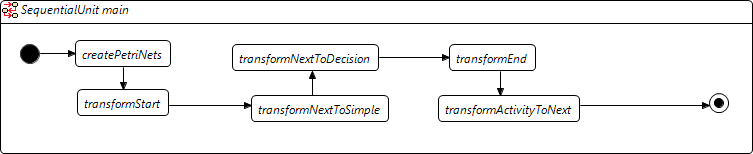
\includegraphics[scale=0.5]{figures/SequentialUnitHenshin.png}
	\caption{A SequentialUnit main that contains a sequence of rules.}
	\label{fig:SequentialUnitHenshin}
\end{figure}

If applicable a transformation unit can also consist of other units, for example
if the user want to either iterate or loop through a transformation rules. This
can also be done with the use of a multi-rule, but in some cases this can only
be done by a LoopUnit or a IterateUnit. Henshin also has two other units that
can administrate transformation rules, namely ConditionalUnit and PriorityUnit.
The ConditionalUnit follows a if-else pattern, and is used if the user want
Henshin to choose between other units. 

\subsection{Translating the instance model}

Now that we have defined the source and target metamodel, created a set of
transformation rules and initialized a control mechanism for these rules it is
time to apply this transformation. For Henshin there is two ways to do this. In
Henshin the default engine for executing model transformation is the Henshin
interpreter. This interpreter can be invoked either by using the a Eclipse wizard
or programmatically using the Henshin API. 

Using the Eclipse wizard this is done by opening the Henshin file in the Henshin
Model Editor and right clicking the root object and locate apply transformation.
This will open a wizard where the user can choose a transformation unit. This
will either be a single transformation rule or some transformation unit that
applies all other units and rules. The user also has to select the instance
model and can explicitly set parameters for the rules if this is applicable. If
the parameter is set to Ignore then the interpreter will automatically match the
parameter. Now the user has two choices, the first choice is to preview the
result of the model transformation. This will either show the user a new window
with the modifications to the model or a message that the rule or unit could not
be applied. If the user press Transform instead of Preview, the model will be
transformed and saved.

The interpreter can also be invoked programmatically, either as an IApplication
in Eclipse or as a simple Java application. Henshin provides a API that lets the
users invoke the interpreter through the use of Java code. There is a class
HenshinResourceSet that lets the user load and save models and transformations.
When the instance model and Henshin module is loaded into the resource set, the
transformation can be applied through the use of the Henshin Engine class. This
is where Henshin finds and translates matches found in the instance graph. The
user also has to specify the main transformation unit from the Henshin module.
Both the engine and the unit can be loaded into the UnitApplication class. And
this class has a method called execute that lets the user execute the model
transformation. If the transformation was executed without errors, then the
instance model can be saved with the translated changes. The Henshin API lets
other users use the power of Henshin in their own program.

\section{Evaluation}
\noindent
Now that we have worked with these tools, we have to evaluate them.
The table underneath summaries the comparison of the different tools, and we
will explain some of them in further detail. We should start talking about how
easy or hard these tools were to learn. It took some time to fully understand
how graph transformations work. That there are a right hand and a left hand
side of each rule, and that these rules also can have both negative and
positive application conditions. But after a while, when the aspects around
graph transformation got clearer, the tools were easier to handle. 

\subsection{The Three Editors}
AGG was the first tool i encountered, my learning curve became steep after i
learned how graph transformations works. AGG has a clear procedure on how to create and
manage new application rules. AGG is also very intuitive to work with, as long
as the users understands the principles behind graph transformation.
After spending time on AGG and its graphical editor to create transformation rules, the next
stop was Henshin. It was difficult to understand how the principles in graph
transformation works in Henshin. The experience with graph transformation from
AGG was not helpful in the initial hours spent on Henshin. The graphical editor
that AGG and Henshin provides are different in such a way that the creation of
rules are different. Both Henshin and AGG has a tree based editor, but the
editor works differently amongst the two tools, see
figure~\ref{fig:AGGTreeBasedEditor} and~\ref{fig:Henshin_TreeEditor} for the
two editors. The tree based editor for AGG is meant to work as a tool for
browsing through the user created rules, application conditions and graphs. And
for each rule in AGG, the graphical editor opens a left hand side and a right
hand side editing part. This is convenient since editing is now separated in a
left hand and a right hand side window in the graphical editor. The graphical editor can also
add a third editing window, if the user has application conditions attached to a
rule. 

For Henshin this is different, because for this tool the graphical editor
is only an extension to make rule management more intuitive for the users. This
graphical editor is stored in a separate file and is synchronized with the main
henshin file. Changes made to one of these two files is synchronized
accordingly to the other file. The main henshin file contains a tree based
editor that is called Henshin Model Editor. And the Henshin users can create and
apply textual transformation rules in this editor without even initialising the
graphical editor. The graphical editor for Henshin does not implicitly provide
any LHS or RHS for the user to edit their rules in. The users have to know how the tool
performs when using the different action types that Henshin provides. This is
different from AGG, where each rule is provided with an own part for editing
both the LHS and the RHS. The Henshin Model Editor updates the RHS and the LHS
explicitly depending of which action type is provided from the graphical
editor when creating nodes and edges. But other than creating and managing
rules both AGG and Henshin are very similar. They both provide a graphical editor where
the users can insert elements that conform to a metamodel. For AGG these
metamodels are represented as a type graph in the tree based editor. While in
Henshin these metamodels are imported to the Module element in the Henshin Model
Editor and synchronized with the graphical editor file.

The third transformation tool we encountered is ATLAS Transformation Language.
And while this tool is definitely not as intuitive as the two graph
transformation tools, once you understand how to create transformation rules
and how to work with the included metamodels, it is a good framework for
working with model transformations. However, if a user do not fully understand
the Object Constraint Language (OCL), ATL is rather a hard tool to work with.
Because OCL has a very leveled learning curve, since it is a declarative
programming language. Where we are more or less used to work with imperative
programming languages during our studies here in Bergen. ATL provides an editor
where the users can use OCL to create and modify transformation rules. ATL has
a very strict way of writing transformation rules, since the tool uses a
textual based approach to create transformation rules. The user has to use the
predefined stereotypes defined by ATL.

\subsection{The Metamodels}
Metamodels are initialised and handled differently amongst some of the tools.
The initialisation of the metamodels for Henshin and ATL is similar. Both of
these tools use Ecore to create metamodels, since they are both integrated with
EMF. For Henshin and ATL the user has to create one Ecore model for both the
source and the target metamodel. Both of these metamodels can be imported both
into Henshin and ATL. One thing that is convenient with Henshin that ATL does
not provide, is that Henshin provides a list of metamodels that is available
for the user. These are metamodels that can be used either as source or target
metamodel. If we want to translate a instance model to an Ecore model, we can
in Henshin import this ecore metamodel from a list and use it as the target metamodel.

Unlike Henshin and ATL, AGG does not allow for separately initialisation of
metamodels. For AGG we have to create both the target and source metamodel in a
disjoint metamodel, or one common type graph in AGG.

The user has to fill out a configuration form for an ATL model transformation.
This form the user has to explicitly assign the metamodels to source model and
target models. The run configuration is done prior to the execution of the model
to model transformation. In Henshin the user has to implicit include the
metamodels in the Henshin module element. Henshin will not allow the user to
create nodes or create edges between nodes that are not defined in the
metamodels. 

AGG on the other hand uses a disjoint metamodel. This means that in AGG there
is something called a type graph, and in this type graph both the target and
the source metamodel are defined. AGG handles consistency similar to
Henshin. AGG will restrict the user to only create nodes or arrows between
nodes that are specified in the type graph. Figure \ref{fig:AggTypeGraph}
in chapter 3 shows that there are created references between two metamodels. And
through the use of these references, AGG can create and modify application
rules to translate these two models represented in the type graph. 
 
\subsection{Transformation Rules}
We have seen that the creation of transformation rules varies over the three
different tools. ATL provides a textual based approach and therefore requires
multiple lines of code. The abstract syntax for the three different tools are
not that different, since both Henshin and ATL utilizes the Ecore model to
create metamodels and AGG creates one type graph that contains the abstract
syntax for both the source and target model. The abstract syntax can be
visualized either by using the tree based model editor that EMF provides or by
using a tird party tool for a graphical representation of the models. The
concrete syntax are obviously different between the three tools. AGG and Henshin
provides a concrete graphical syntax, while ATL on the other side provides a
concrete textual syntax for creating and modifying transformation rules. For
both AGG and Henshin the rules can be created and modified by using a graphical
editor. AGG separates the RHS and the LHS in two separate editing parts while
Henshin use predefined word sequences to distinguish the two different sides.
If the rules are quite large, with multiple nodes and arrows the rules
presented in Henshin becomes easier to read and maintain. But both AGG and
Henshin has a clear way of representing the rules and possible attached
application conditions. All three tools have a left hand side
and a right hand side, but are represented differently amongst the rules.
Henshin and AGG use graph patterns to represent the LHS and the RHS while ATL
utilizes logical expressions. In section 3 we discussed that ATL can have both
declarative and imperative transformation rules. In Henshin and AGG the LHS and
the RHS are represented as graphs. Where the LHS represents the pattern graph
that is matched for an instance model and the RHS represents the part that should be
replaced for the instance model. For ATL the LHS represents the source model
while the RHS represents the target model. 

Both AGG and Henshin can specify both negative and positive application
conditions. These are attached to pattern graph or the LHS of a rule. These
application conditions provides a true or false clause that can be used to
restrict the pattern graph. For ATL these conditions are handled by OCL
expressions, where one example is the if-then clause.

\subsection{Relationship between Source and Target}
For an exogenous transformation in ATL it is mandatory to create a new target
that holds all the target model elements. Exogenous model transformation in ATL
is therefore called an out-place transformations. In AGG on the other hand both
source and target model is always the same model. This means that AGG performs an
in-place update on its original source model. Henshin is a bit more special,
because implicitly it performs in-place update on the source model. But in
Henshin you can initialize variables that explicitly captures the transformed
target elements and save these to a separate file in your storage unit. Note
however, that this can only be done when utilizing the Henshin interpreter
programmatically. 

\subsection{Rule Scheduling}

ATL has does the scheduling implicit, where the user has no control over the
scheduling algorithm defined by the tool. The user can however influence the scheduling
algorithm defined by the ATL transformation engine by designing the logic in the
transformation rules to apply in a certain order. The transformation
engine will first execute the declarative rules before applying the imperative
section of a transformation rule. AGG and Henshin does however, give the
users the possibility to influence how the transformation rules are applied. 
In Henshin and AGG this is handled explicitly before applying the transformation
rules, where the user can change the execution order of the rule.
For example the rules can be applied non-deterministically or by forcing the
transformation rules to be applied in a sequential order. To force the
transformation in a sequential order could result in performance issues compared
to applying the rules non-deterministically. AGG provides the users with the
possibility to organize the transformation process into several phases or
layers. These layers are numbered from 0 \ldots n, and the lower the number the
higher the priority for the rule, when it is translated. This gives the users
the possibility to execute rules layer by layer. In Henshin these rule scheduling
mechanisms are referred to as transformation units. For this tool it is possible
to specify units that supports rule iteration, both by looping through rules
until there are no more changes detected or by iterating through rules for a
fixed number of iterations. In Henshin it is also possible to specify an
amalgamation unit, that is an unit that provides a forall-operation for the
matching pattern graph. This unit has a kernel rule and multiple underlying
rules that are matched as often as possible. This amalgamation unit can be
compared to a for loop in Java. It is clear that Henshin provides the users with
quite an variety of controlling the execution of rules.

\subsection{Rule Organization}

ATL organizes the transformation rules inside modules, and its therefore easy to
reuse these modules if applicable. This is convenient for
users of ATL since this means that all created rules can be used to form new
transformation rules. Henshin provides the user with the possibility to nest or 
reuse rules in different scheduling mechanism or transformation units
as we discussed in the last paragraph. But Henshin and AGG does however not
provide the user with the possibility to reuse rules in the creation of new
rules as ATL does. 

\subsection{Tracing}

Tracing in the three tools provides a unique link
between a source and a target. The source represents the matched part while the
target represents the generated or replacement part. All three tools provides
dedicated support for traceability. But these traceable links are handled
differently amongst the tools. For ATL the trace model works as a storage
location and automatically creates trace links between source and target
elements. These traceable links are internally used by the ATL
transformation engine when executing a model transformation. But we explained in
section 3 that these trace links can be explicitly captured by creating
transformation rules that generates a collection of trace links in a
separate trace file. Henshin does this differently, because tracing is
controlled by the users. Henshin has a dedicated Trace Model that can be
imported to the Henshin module as an Ecore model. The trace model in Henshin
are automatically created when executing rules, but the user have to manually
assign the traceable links inside the transformation rules. The traces in
Henshin are translated when a rule is executed, and therefore the user has to
be aware of this when using these traces in other rules, since this
could lead to the creation of multiple traceable links between the same
elements. Tracing in AGG plays a vital role to executing model transformations.
Traceable elements are created similar to any other elements when initializing
the type graph. With traceable links between the source and the
target elements, AGG can be certain that elements are transformed. The traceable
link in AGG ensures that a match in the pattern graph is only matched once. If we do
not create a traceable link between source and target elements in AGG, the
rules will be applied an endless amount of times. Tracing amongst the three
different tools are different in such a way that it is required for exogenous
model transformations for AGG and ATL. In ATL the traceable links are created
automatically and cannot be controlled by the users, while in AGG the traceable
links are created as bridges between source and target elements. For Henshin
the Trace model is optional. 

\subsection{Directionality}

Its clear to see that all three tools are unidirectional, since they can be
executed in one direction only. And that is to compute a target model from a
source model. The three tools requires two model transformations to be able to
transform in multiple directions. Where the source and target model and
metamodels switch places. But this is not how multidirectional transformations
work. A multidirectional transformation can execute in both direction when
performing a model transformation.

\begin{table}[ht]
\centering
\begin{tabular}{| c | c | c | c |}
\hline
 & AGG & Henshin & ATL \\
\hline
Endogenous transformation & \cellcolor{green!25}Yes &
\cellcolor{green!25}Yes & \cellcolor{green!25}Yes \\

Exogenous transformation & \cellcolor{green!25}Yes &
\cellcolor{green!25}Yes & \cellcolor{green!25}Yes \\

Input Elements & 1\ldots n & 1\ldots n & 1\ldots n\\
Output Elements & 1\ldots n & 1\ldots n & 1\ldots n\\
Graphical editor &\cellcolor{green!25}Yes &
\cellcolor{green!25}Yes &\cellcolor{red!25}No  \\
Integrated with Java & \cellcolor{green!25}Yes &
\cellcolor{green!25}Yes & \cellcolor{green!25}Yes \\
Separate metamodels & \cellcolor{red!25}No &
\cellcolor{green!25}Yes & \cellcolor{green!25}Yes \\
Integrated with EMF & \cellcolor{red!25}No &
\cellcolor{green!25}Yes & \cellcolor{green!25}Yes \\
Model transformation file size &200 kb &80 kb &4 kb \\
In-place/out-place model transformation &in-place &
in-place &out-place \\
\hline

\end{tabular}
\caption{Comparing model transformation tools.}
\end{table}

\newpage

From the table above, we can see that all the three tools have support
for both endogenous and exogenous model transformations. 

All the three tools has support for an arbitrary number of both input and
output elements. This means that if the tool takes a number of input models, then it
produces the same number of target models. Take an ATL module as an example. It
accepts a fixed number of models as input, and returns a fixed number of target
models. This means that an ATL module can not generate an unknown number of
target models. If there is one input model, then there will be one output model
that conforms to a target metamodel.

Both AGG and Henshin provides a graphical editor, where the users can create and
modify transformation rules. This makes them both very intuitive for the users.
This is not the case for ATL, which uses a textual based approach. For ATL the
users have to implement transformation rules in programming code.

All three tools can be integrated with Java. For Henshin and ATL the files
containing the transformation rules have to be created before they can be used
in a java application. In ATL this has to be a ``atl'' file containing a ATL
module that has a list of rules. This is because the ATL transformation engine
relies on a file extension with the name ``atl''.

One thing that is worth mentioning is that AGG does not support the Eclipse
Modelling Framework. In EMF the root of all modelling objects is called
EObject. And this EObject has no references to the Java Object. Therefore AGG
can not be integrated with EMF, since AGG can take Java Objects as input,
but not EObjects. Both Henshin and ATL supports EMF. This means that the user
can use the EMF API together with Henshin and ATL in a Java Application.

We can also se that the size of the transformation rules is different
between the three tools. A classic example of an exogenous transformation is
translating from a class diagram to a relational database, that has more or less become a
benchmark for model to model transformations. For this example we can see that
AGG uses 200 kb of the storage space. This number is so unbelievable small
that it will never be noticed in any modern computers. But there is one
interesting thing however, and that is that the transformation rules defined in
ATL is 50 times smaller than AGG. What this basically means is that creating model
transformations through the use of textual concrete syntax is less space
consuming than through the use of graphical syntax. This is only logical since
the graphical syntax based transformation languages requires more storage
space simply because they use graphical elements to represent the transformation
rules.

\subsection{Translating the instance model}

When ATL transformation language executes the application rules for the model to
model transformation, a new model instance is created for the target model. This
means that the source model is independent of the target model. Where Henshin
and AGG performs in-place model to model transformations. This means that they
both operate on an instance model of the source metamodel, and translates
inside this instance model. All three approaches can however give the same
result. Inn AGG and Henshin the users just need to make sure to delete unwanted
elements from the translated host graph. On the other side, for ATL this is not
needed, since both the source and target model are kept as separated files. This
is also possible to achieve with Henshin. If the user programmatically invoke
the Henshin Interpreter the target model can be forced to be saved in a newly
created file. Henshin will still do an in-place model transformation, but it is
possible to save the translated object in a separate file. It is then possible
to perform an in-place transformation in Henshin while saving the target
instance model in a separate file. 

\subsection{Conclusion}

We have experienced that after working with the three tools that in the initial
learning phase both AGG and Henshin seems to be more intuitive to use because of the
graphical editor they provide. Because of the extensive language OCL, ATL
requires more hours to understand compared to AGG and Henshin. Its important to
take into consideration that I have read through papers that explain the
principles behind graph transformations. This makes it easier to understand how
AGG and Henshin introduces the users to model transformation, even though both
tools have different solutions to how graph transformation is implemented. But
learning a new programming language requires time. And therefore a graphical
solution might feel more intuitive then a textual solution. However I also know
that if you master a programming language, then writing code is more productive
compared to using a graphical editor. Therefore if the user master both the ATL
transformation language and the OCL programming language then it might be a
productive way of creating transformation rules. All these three tools have gone
through several iterations and releases and also have received feedback from the
user community. This only reassure me that all these three tools are viable
choices for model transformations. Most of the hours have been spent on
Henshin's working with the graphical editor and programmatically
invoking the Henshin interpreter. The graphical editor provides a clear
process of defining new transformation rules once I understood how the graph
transformation principles worked for Henshin. The Henshin Interpreter has
an extensive API that can be used to programmatically translate the
models. The interpreter still requires a set of Henshin rules to be able to
initiate a model transformation, but this means that the user can create its own
graphical editor and integrate this editor with Henshin to manipulate models.
Together with the Henshin Model Editor, the graphical editor and the Henshin
Interpreter Henshin provides a very viable transformation language for model
transformations.

\noindent 

\bibliographystyle{ieeetr} 
\bibliography{master,websites}

\end{document}